% yaml_data_model.tex
% Data model / storage structure diagram
% Author: João Pedro Azevedo
% Date: December 2025

\documentclass[tikz,border=10pt]{standalone}
\usepackage{tikz}
\usetikzlibrary{shapes.geometric, arrows.meta, positioning, fit, backgrounds, calc, matrix}

\begin{document}

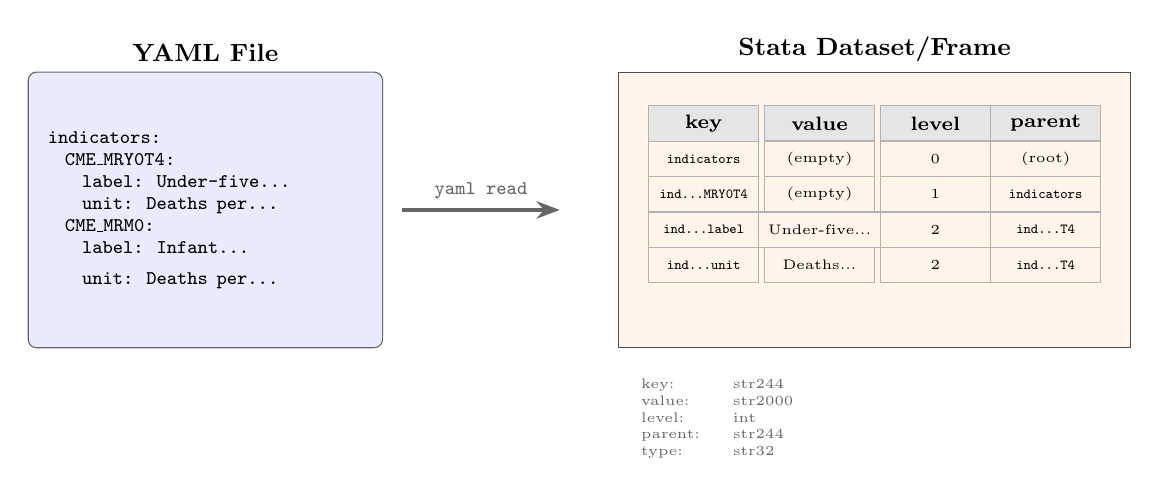
\begin{tikzpicture}[
    % YAML file style
    yamlfile/.style={
        rectangle, 
        rounded corners=3pt,
        draw=black!60, 
        fill=blue!8,
        minimum width=4.5cm, 
        minimum height=3.5cm,
        font=\small,
        align=left
    },
    % Dataset style
    dataset/.style={
        rectangle, 
        draw=black!70, 
        fill=orange!8,
        minimum width=6.5cm, 
        minimum height=3.5cm,
        font=\small
    },
    arrow/.style={
        ->,
        >=Stealth,
        very thick,
        black!60
    },
    label/.style={
        font=\small\bfseries
    }
]

% === YAML File (Left) ===
\node[yamlfile, text width=4cm] (yamlfile) at (0, 0) {
    {\ttfamily\scriptsize
    indicators:\\
    \ \ CME\_MRY0T4:\\
    \ \ \ \ label: Under-five...\\
    \ \ \ \ unit: Deaths per...\\
    \ \ CME\_MRM0:\\
    \ \ \ \ label: Infant...\\
    \ \ \ \ unit: Deaths per...
    }
};
\node[label, anchor=south] at (yamlfile.north) {YAML File};

% === Arrow ===
\draw[arrow] (2.5, 0) -- node[above, font=\scriptsize\ttfamily] {yaml read} (4.5, 0);

% === Stata Dataset (Right) ===
\node[dataset] (dta) at (8.5, 0) {};
\node[label, anchor=south] at (dta.north) {Stata Dataset/Frame};

% Table inside dataset
\matrix[matrix of nodes, 
        nodes={rectangle, draw=black!30, minimum width=1.4cm, minimum height=0.45cm, font=\scriptsize, anchor=center},
        column sep=-\pgflinewidth,
        row sep=-\pgflinewidth,
        ampersand replacement=\&] at (8.5, 0.2) {
    |[fill=gray!20, font=\scriptsize\bfseries]| key \& 
    |[fill=gray!20, font=\scriptsize\bfseries]| value \& 
    |[fill=gray!20, font=\scriptsize\bfseries]| level \& 
    |[fill=gray!20, font=\scriptsize\bfseries]| parent \\
    |[font=\tiny\ttfamily]| indicators \& 
    |[font=\tiny]| (empty) \& 
    |[font=\tiny]| 0 \& 
    |[font=\tiny]| (root) \\
    |[font=\tiny\ttfamily]| ind...MRY0T4 \& 
    |[font=\tiny]| (empty) \& 
    |[font=\tiny]| 1 \& 
    |[font=\tiny\ttfamily]| indicators \\
    |[font=\tiny\ttfamily]| ind...label \& 
    |[font=\tiny]| Under-five... \& 
    |[font=\tiny]| 2 \& 
    |[font=\tiny\ttfamily]| ind...T4 \\
    |[font=\tiny\ttfamily]| ind...unit \& 
    |[font=\tiny]| Deaths... \& 
    |[font=\tiny]| 2 \& 
    |[font=\tiny\ttfamily]| ind...T4 \\
};

% === Storage types annotation ===
\node[font=\tiny, text=black!60, anchor=north west] at (5.2, -2) {
    \begin{tabular}{ll}
    key: & str244 \\
    value: & str2000 \\
    level: & int \\
    parent: & str244 \\
    type: & str32
    \end{tabular}
};

\end{tikzpicture}

\end{document}
